\documentclass{beamer}\usepackage[]{graphicx}\usepackage[]{xcolor}
% maxwidth is the original width if it is less than linewidth
% otherwise use linewidth (to make sure the graphics do not exceed the margin)
\makeatletter
\def\maxwidth{ %
  \ifdim\Gin@nat@width>\linewidth
    \linewidth
  \else
    \Gin@nat@width
  \fi
}
\makeatother

\definecolor{fgcolor}{rgb}{0.345, 0.345, 0.345}
\newcommand{\hlnum}[1]{\textcolor[rgb]{0.686,0.059,0.569}{#1}}%
\newcommand{\hlstr}[1]{\textcolor[rgb]{0.192,0.494,0.8}{#1}}%
\newcommand{\hlcom}[1]{\textcolor[rgb]{0.678,0.584,0.686}{\textit{#1}}}%
\newcommand{\hlopt}[1]{\textcolor[rgb]{0,0,0}{#1}}%
\newcommand{\hlstd}[1]{\textcolor[rgb]{0.345,0.345,0.345}{#1}}%
\newcommand{\hlkwa}[1]{\textcolor[rgb]{0.161,0.373,0.58}{\textbf{#1}}}%
\newcommand{\hlkwb}[1]{\textcolor[rgb]{0.69,0.353,0.396}{#1}}%
\newcommand{\hlkwc}[1]{\textcolor[rgb]{0.333,0.667,0.333}{#1}}%
\newcommand{\hlkwd}[1]{\textcolor[rgb]{0.737,0.353,0.396}{\textbf{#1}}}%
\let\hlipl\hlkwb

\usepackage{framed}
\makeatletter
\newenvironment{kframe}{%
 \def\at@end@of@kframe{}%
 \ifinner\ifhmode%
  \def\at@end@of@kframe{\end{minipage}}%
  \begin{minipage}{\columnwidth}%
 \fi\fi%
 \def\FrameCommand##1{\hskip\@totalleftmargin \hskip-\fboxsep
 \colorbox{shadecolor}{##1}\hskip-\fboxsep
     % There is no \\@totalrightmargin, so:
     \hskip-\linewidth \hskip-\@totalleftmargin \hskip\columnwidth}%
 \MakeFramed {\advance\hsize-\width
   \@totalleftmargin\z@ \linewidth\hsize
   \@setminipage}}%
 {\par\unskip\endMakeFramed%
 \at@end@of@kframe}
\makeatother

\definecolor{shadecolor}{rgb}{.97, .97, .97}
\definecolor{messagecolor}{rgb}{0, 0, 0}
\definecolor{warningcolor}{rgb}{1, 0, 1}
\definecolor{errorcolor}{rgb}{1, 0, 0}
\newenvironment{knitrout}{}{} % an empty environment to be redefined in TeX

\usepackage{alltt}
\IfFileExists{upquote.sty}{\usepackage{upquote}}{}
\begin{document}

\begin{frame}
\frametitle{Exercício 1}
Praticando o Latex
\end{frame}

\begin{frame}
\frametitle{Texto}
1. Usando o formato “.Rnw”, crie um PDF com texto simples usando pelo menos cinco das formatações acima (bold, itálico, etc.).

\textbf{Bold} 
\textit{Itálico}
\underline{Underline}
\section{Titulo 1}
\subsection{Subtitulo 1}
\subsubsection{Subsubtitulo 1}
\end{frame}

\begin{frame}
\frametitle{Equação}
2. Adicione a famosa equação do teorema de Pitágoras no seu documento.

\begin{equation}
a^2 = b^2 + c^2
\end{equation}
\end{frame}

\begin{frame}[fragile]
\frametitle{Tabela}
3. Adicione uma tabela simples no PDF usando o banco de dados de weather, resumindo o total de precipitação por mês.


\begin{tabular}{r|r}
\hline
month & atraso\_medio\\
\hline
1 & 10.036665\\
\hline
2 & 10.816842\\
\hline
3 & 13.227076\\
\hline
4 & 13.938038\\
\hline
5 & 12.986859\\
\hline
6 & 20.846332\\
\hline
7 & 21.727787\\
\hline
8 & 12.611040\\
\hline
9 & 6.722476\\
\hline
10 & 6.243988\\
\hline
11 & 5.435362\\
\hline
12 & 16.576688\\
\hline
\end{tabular}


\end{frame}

\begin{frame}[fragile]
\frametitle{Gráfico}
4. Adicione um gráfico simples usando o banco de dados weather, ilustrando temperatura média por aeroporto.

\begin{knitrout}
\definecolor{shadecolor}{rgb}{0.969, 0.969, 0.969}\color{fgcolor}
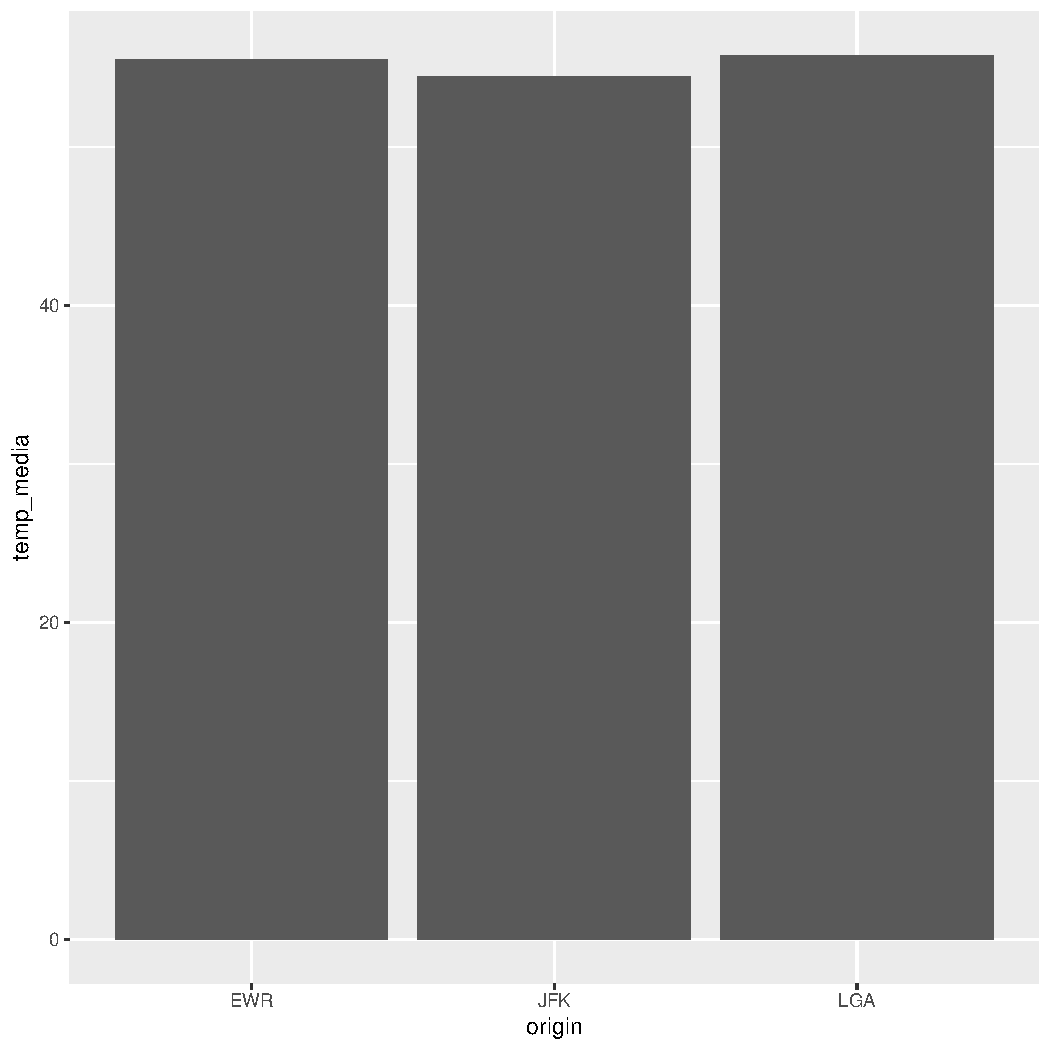
\includegraphics[width=\maxwidth]{figure/unnamed-chunk-2-1} 
\end{knitrout}
\end{frame}

\begin{frame}
5. Verifique que o seu documento compila sem erro para PDF.

Feito!
\end{frame}

\begin{frame}
6. Ajuste o seu script “.Rnw” acima para gerar uma apresentação do class ‘beamer’ e coloque o texto, a equação, a tabela, e o gráfico em slides diferentes. Compile para PDF de novo.
\end{frame}

\begin{frame}
\frametitle{Exercício 2}
Usando Git
\end{frame}

\begin{frame}
\frametitle{1}
Crie um novo repositório na sua conta de Github e conecte (‘clonar’) com um novo projeto no seu RStudio.

Feito!
\end{frame}

\begin{frame}
\frametitle{2}
Copie o seu script de Exercício 1 acima (o .Rnw) para a pasta local do seu projeto novo criado no passo anterior.

Feito!
\end{frame}

\begin{frame}[fragile]
\frametitle{3}
Adicione mais um gráfico ao seu script, mostrando a umidade média por mês do banco de dados de weather.

\begin{knitrout}
\definecolor{shadecolor}{rgb}{0.969, 0.969, 0.969}\color{fgcolor}
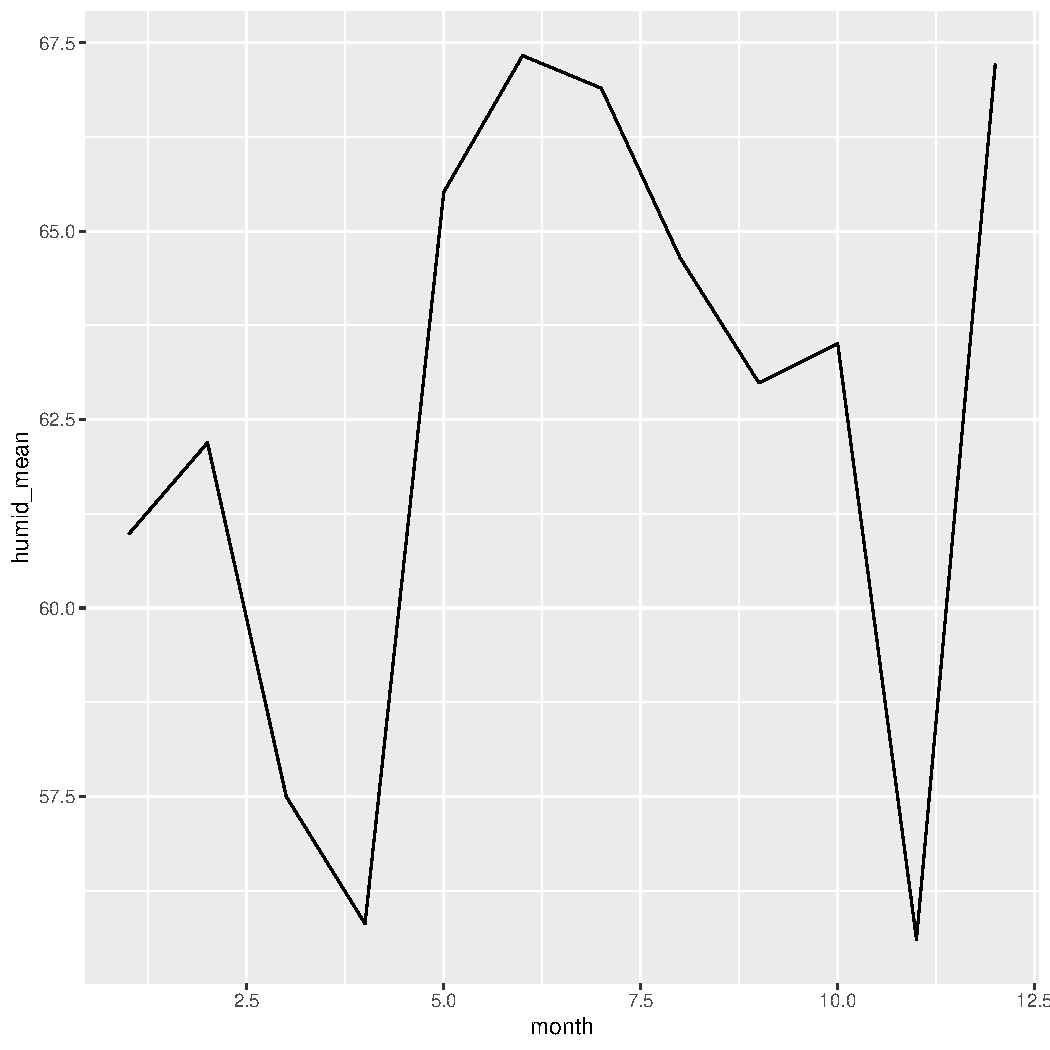
\includegraphics[width=\maxwidth]{figure/unnamed-chunk-3-1} 
\end{knitrout}

\end{frame}

\begin{frame}
\frametitle{4}
Usando a aba de Git, execute Commit com a versão atualizada do script Rnw, atribuindo uma descrição apropriada.

Feito!
\end{frame}

\begin{frame}
\frametitle{5}
Execute Push das mudanças para o seu repositório do Github online. Verifique que o novo arquivo está atualizado no repositório da sua conta deo Github.

Feito!
\end{frame} 























\end{document}
